\section{Ginocchio (Pogliacomi)}

L'articolazione del ginocchio è un'articolazione che, dal punto di vista anatomico e biomeccanico, può essere considerata una doppia articolazione condiloidea fra i due condili del femore e i due piatti tibiali, a cui si associa poi l'articolazione trocleare fra la troclea
femorale e la rotula.
L'articolazione del ginocchio dal punto di vista osseo non è particolarmente stabile, ossia la convessità dei condili femorali non corrisponde precisamente con la concavità dei due piatti tibiali.
(Al contrario a livello dell'anca la congruenza articolare è particolarmente importante, la testa del femore forma una sorta di vuoto con l`acetabolo.)

Per dare stabilità a questo tipo di articolazione subentrano degli elementi stabilizzatori passivi e degli elementi stabilizzatori attivi. Attivi sono i gruppi muscolari la cui contrazione rinforza l'articolazione, tra questi vanno ricordati:

\begin{itemize}
\item
  i tendini del semimembranoso e i tendini della zampa d'oca medialmente
\item
  il sistema quadricipite-rotula-tendine rotuleo anteriormente,
\item
  il tendine del bicipite femorale in posizione laterale
\item
  i gastrocnemi in posizione posteriore.
\end{itemize}

Mentre i passivi sono la capsula e i legamenti. La capsula è essenzialmente un manicotto fibroso che unisce il femore alla tibia, rinforzata da diversi legamenti, cioè fasci di tessuto fibro-collageno denso, simili ai tendini, la cui posizione e disposizione corrisponde alle linee di tensione che entrano in funzione durante i movimenti articolari del ginocchio, ed analoga struttura hanno anche i legamenti crociati. In generale, il ginocchio è un'articolazione complessa, anche se il suo movimento avviene praticamente solo sul piano sagittale, in un meccanismo di flesso-estensione che va da 180\textsuperscript{o} a 30\textsuperscript{o}, e in questo movimento la superficie articolare della tibia ruota su quella del femore, ma il centro di tale rotazione non è fisso, ma tende a spostarsi in dietro col progredire della flessione. Quando il ginocchio è completamente esteso, ogni movimento che non sia di flessione è impossibile, mentre quando il ginocchio è flesso, sono concessi dei movimenti di rotazione della tibia rispetto al femore: nella rotazione interna, i due legamenti crociati si avvolgono tra loro e così la limitano; nella rotazione esterna, invece, si svolgono e la limitazione è allora principalmente affidata alla capsula mediale e al punto d'angolo postero-interno.
\\\\
È importante tenere a mente che, in condizioni normali, le strutture di sostegno dell'articolazione del ginocchio agiscono in modo sinergico tra loro, e la sezione di un solo legamento non produce alcuna instabilità del ginocchio, con l'eccezione del legamento crociato posteriore, la cui sezione determina immediata instabilità articolare, in quanto rappresenta il vero asse portante di questa articolazione. Il legamento crociato posteriore è un legamento robusto, si rompe solo con forze molto intense, e quindi la sua interruzione crea instabilità del ginocchio con sublussazione posteriore della tibia, ma fortunatamente è un legamento extra-articolare e le sue lesioni tendono a cicatrizzare piuttosto bene. Il legamento crociato anteriore, invece, è più fragile, e molto più esposto alla rottura, perché partecipa alla stabilizzazione del ginocchio in tutte le posizioni; una sua interruzione isolata non determina instabilità articolare, ma tale instabilità può comparire in caso di lesioni capsulari mediali o laterali, o se viene tolto il menisco mediale. Le lacerazioni del crociato anteriore tendono a cicatrizzare male, perché è una struttura poco vascolarizzata, e spesso i suoi monconi tendono a sfilacciarsi e a retrarsi.

\subsection{Legamenti}

\begin{figure}[!ht]
\centering
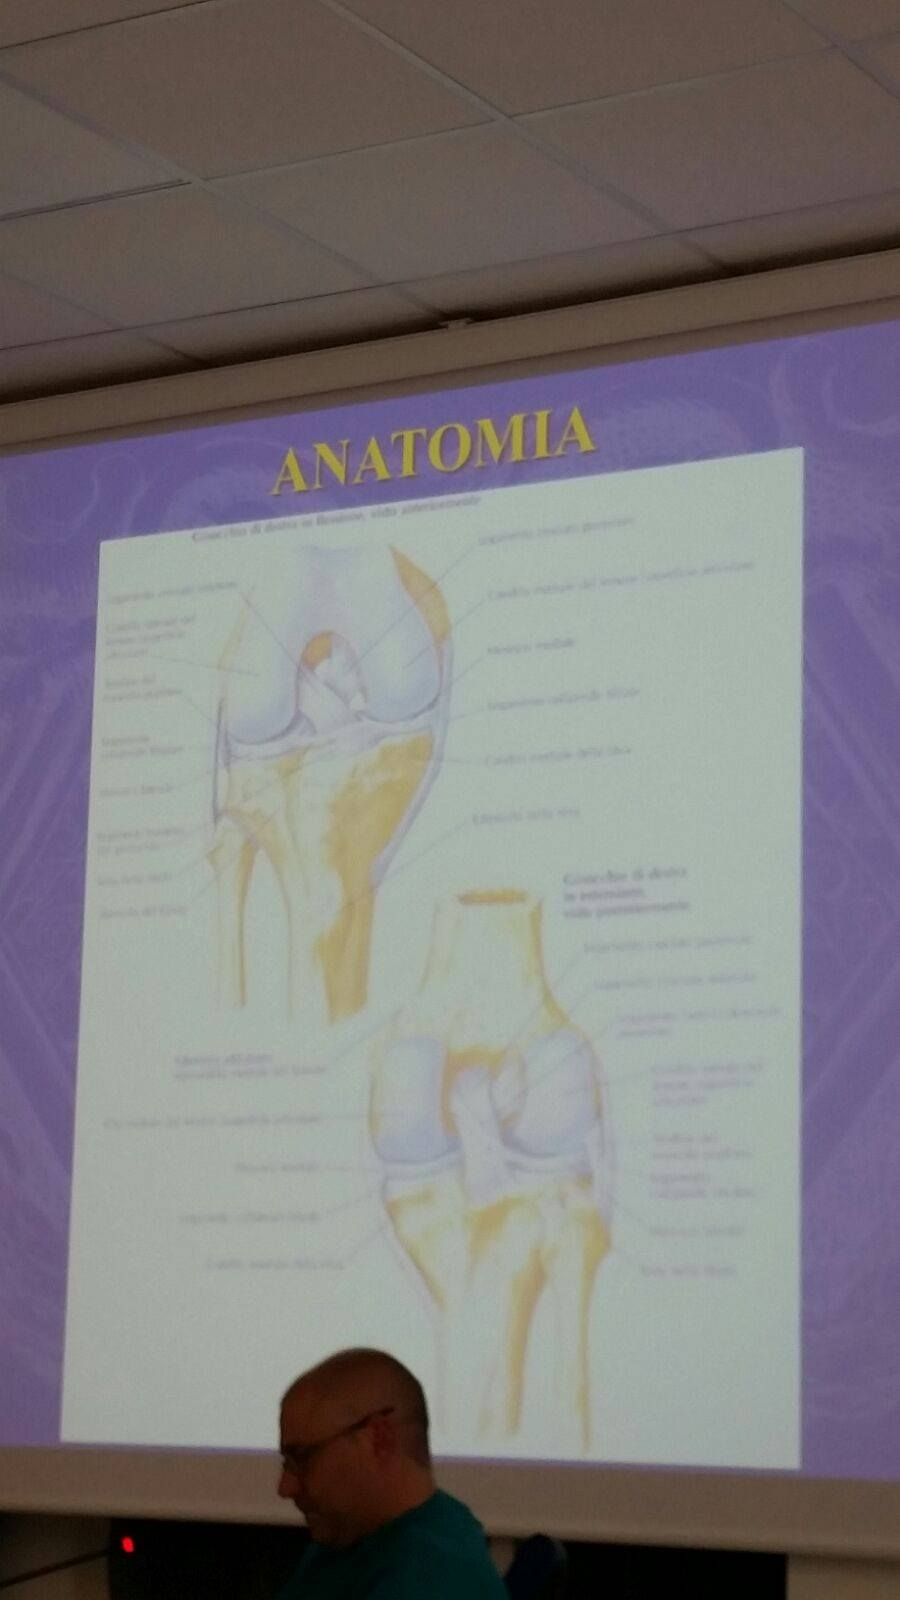
\includegraphics[width=0.4\textwidth]{008/image1.jpeg}
\end{figure}

A livello dell'articolazione i legamenti più importanti sono:
\begin{itemize}
\item[1.] Il \textbf{legamento} \textbf{collaterale mediale}, legamento nastriforme che origina dalla faccia esterna del condilo femorale mediale e si va ad inserire a ventaglio sulla faccia interna dell'emipiatto tibiale mediale. In posizione mediale la capsula è rinforzata anche dalle inserzioni tendinee del semimembranoso e dal
menisco mediale, e questa area prende il nome di ``punto d'angolo postero-interno''
\item[2.] Il \textbf{legamento collaterale laterale}, legamento cordoniforme che origina dalla faccia esterna del condilo femorale laterale e si inserisce in corrispondenza della testa del perone. In posizione
laterale la capsula è rinforzata anche dadalla banderella di Maissiat, che è una prosecuzione della fascia lata e che si inserisce sul tubercolo tibiale di Gerdy), dal legamento popliteo arcuato e dal tendine del muscolo popliteo, e questi ultimi costituiscono quello che prende il nome di ``punto d'angolo postero-esterno''.
Questi due legamenti controllano prevalentemente la \textbf{stabilità medio-laterale} del ginocchio.
In particolare il legamento collaterale mediale si oppone al valgo stress del ginocchio, mentre il legamento collaterale laterale si oppone al varo stress del ginocchio.
\\\\
Legamenti che controllano invece la \textbf{stabilità in senso antero-posteriore e rotazionale} del ginocchio sono rappresentati da:
\item[3.] Il \textbf{legamento crociato antero esterno}, che origina dalla spina tibiale anteriore, si porta in alto, indietro e verso l'est e si va ad inserire sulla faccia mediale del condilo femorale esterno.
\item[4.] il \textbf{legamento crociato posteriore}, che origina dalle spine tibiali posteriori sul piatto tibiale, si porta in alto, in avanti e verso l'interno e si va ad inserire sulla faccia mediale del condilo femorale mediale.
\end{itemize}

\subsection{Menischi}

Oltre ai legamenti a livello dell'articolazione del ginocchio troviamo i menischi, strutture fibrocartilaginee a sezione triangolare. Si interpongono tra i condili femorali e i due emipiatti tibiali e dall'alto hanno la tipica forma di ``C''. Sono all'interno del ginocchio, ma all'esterno della cavità articolare, poiché rivestiti dalla membrana sinoviale. I menischi sono costituiti da tessuti fibro-cartilagineo e privi di vasi nella loro porzione centrale, mentre la loro porzione periferica, più spessa ed unita alla capsula articolare, contiene una modesta vascolarizzazione, da cui ne consegue che solo la parte più esterna dei menischi può eventualmente cicatrizzare.
Hanno una doppia funzione:

\begin{itemize}
\item
  sono ammortizzatori tra i condili femorali e gli emipiatti tibiali e perciò assorbono le forze che si ripercuotono a livello dell'articolazione durante il cammino o la corsa.
\item
  aumentano la congruenza articolare tra i condili e gli emipiatti. (stabilizzatori passivi)
\end{itemize}

Queste capsule legamentose meniscali possono lesionarsi e rompersi durante i traumi distorsivi del ginocchio. Le lesioni meniscali possono essere isolate oppure associate a lesioni legamentose e a loro volta le lesioni legamentose possono essere isolate o associate ad una lesione meniscale. Il menisco mediale è più fisso rispetto al menisco laterale, nel senso che si muove meno nei movimenti di flesso-estensione del ginocchio, ed anche per questa sua caratteristica, è più soggetto alle lesioni nei traumi distorsivi del ginocchio.

\subsection{Assi meccanici e anatomici}

Per capire l'esame obiettivo del ginocchio dobbiamo inquadrare fisiologicamente l'asse dell'arto inferiore. Si parla di asse meccanico e anatomico.

\begin{figure}[!ht]
\centering
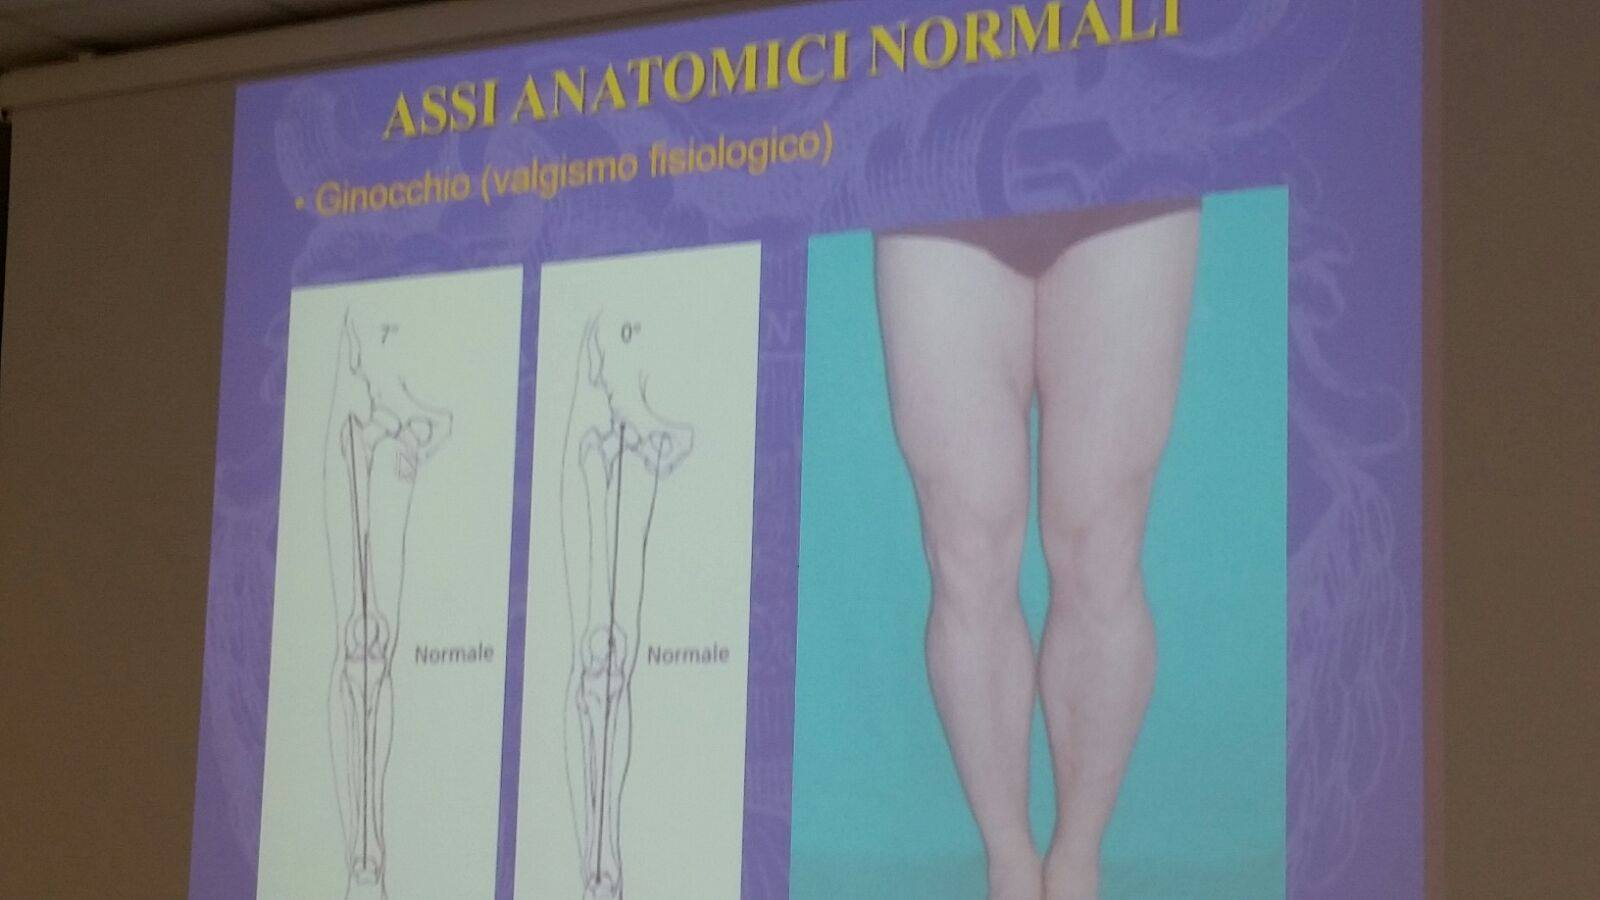
\includegraphics[width=0.4\textwidth]{008/image2.jpeg}
\end{figure}

L'\textbf{asse meccanico} è rappresentato da una retta che parte dal centro della testa del femore e arriva al centro della caviglia. In condizioni di normalità passerà per il centro del ginocchio o appena lateralmente dal centro del ginocchio.
L'\textbf{asse anatomico} è una linea che nasce dall'unione di due rette, una che passa all'interno del canale femorale del femore e arriva al ginocchio e l'altra che passa all'interno del canale femorale della
tibia e arriva al ginocchio. Queste due rette non sono parallele, ma incontrandosi formano l'asse anatomico del ginocchio con un angolo di valgismo fisiologico di circa 173-178 gradi.

\subsubsection{Ginocchio Varo}

\begin{figure}[!ht]
\centering
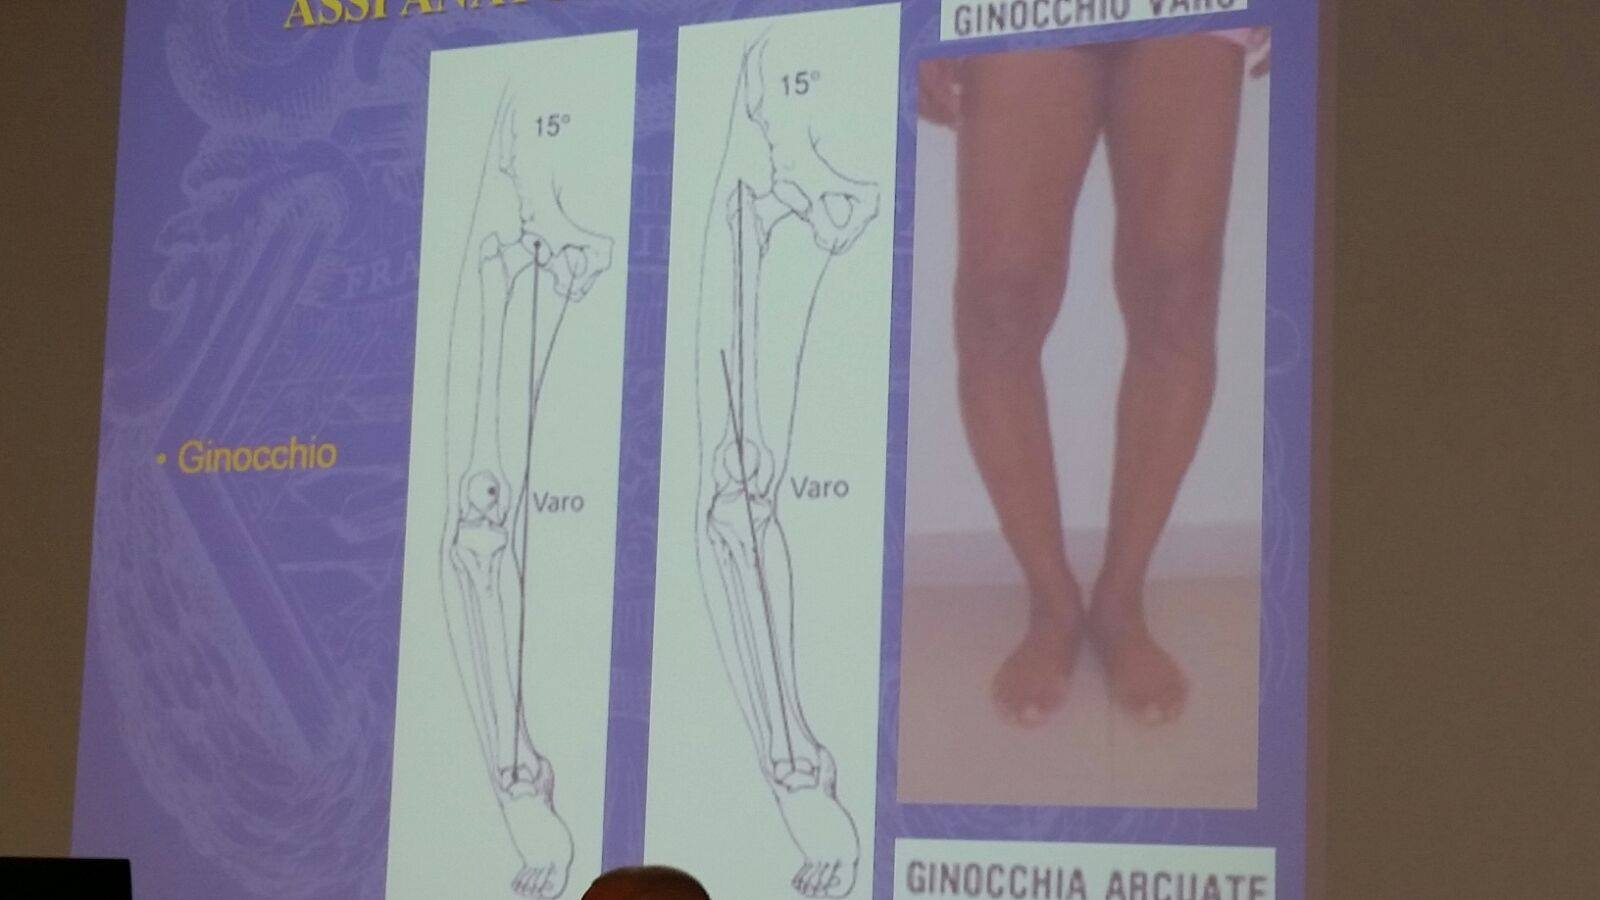
\includegraphics[width=0.4\textwidth]{008/image3.jpeg}
\end{figure}

Si parla di \textbf{ginocchio varo} nel momento in cui vengono alterati gli assi meccanici e anatomici. L'asse meccanico è spostato all'interno del ginocchio e l'asse di valgismo fisiologico sarà superiore ai 178 gradi considerati normali. Detto in maniera semplicistica siamo di fronte al ginocchio a parentesi del calciatore. Questa condizione implica che le forze di carico che agiscono sull'articolazione del ginocchio saranno tutte concentrate nella parte interna del ginocchio stesso. Questo comporterà una maggior usura della cartilagine e una maggior possibilità di andare incontro a degenerazione articolare artrosica precoce.

\subsubsection{Ginocchio Valgo}

\begin{figure}[!ht]
\centering
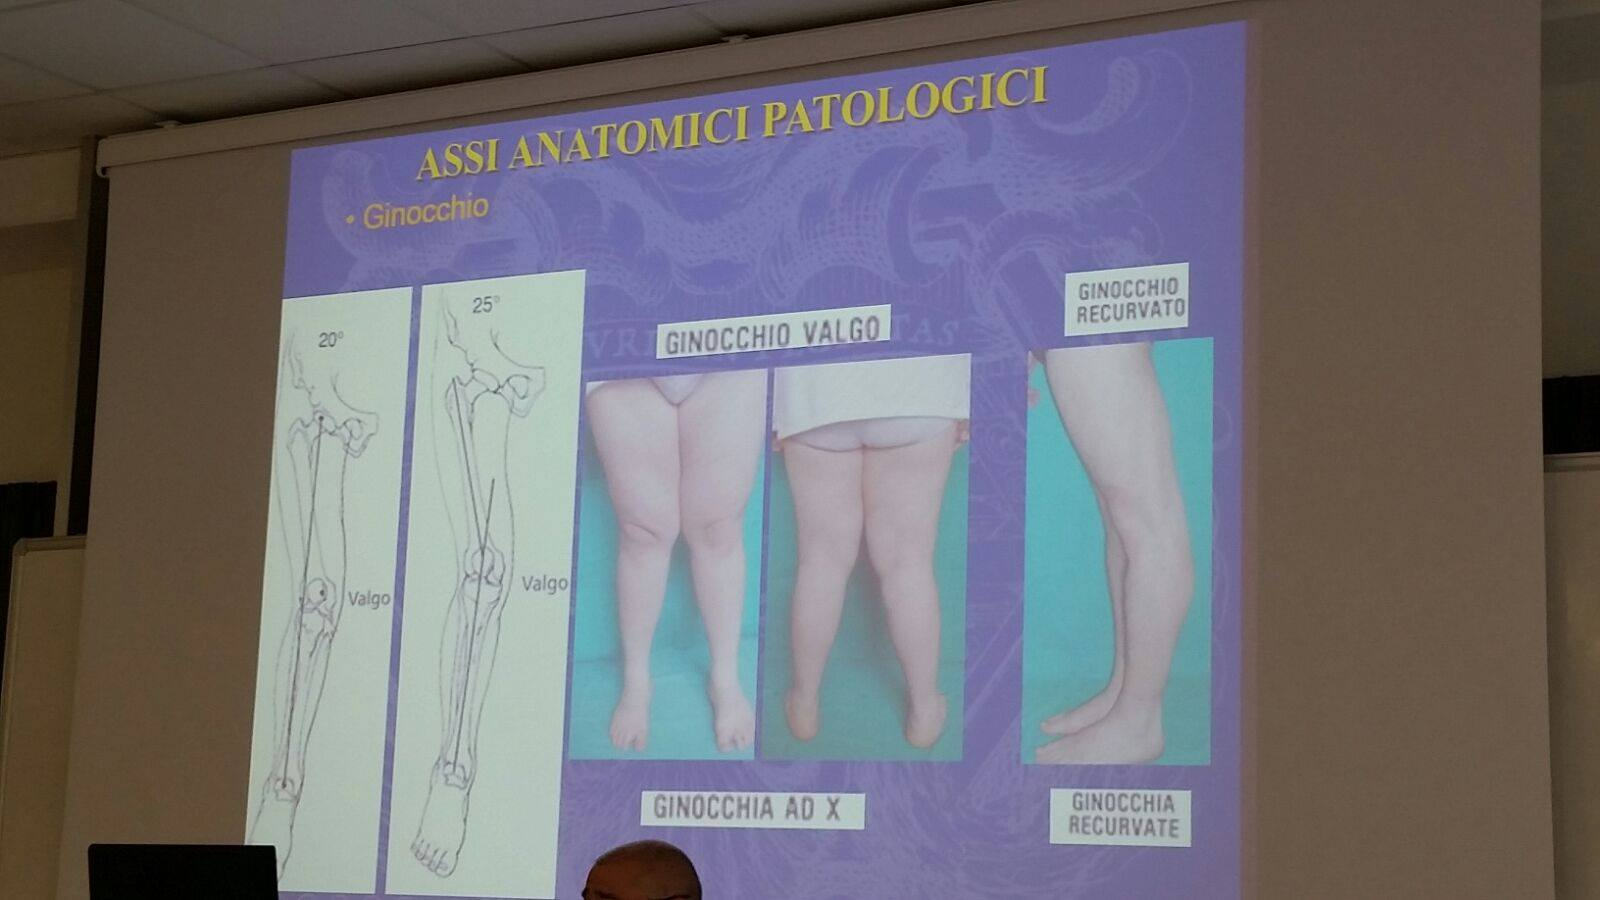
\includegraphics[width=0.4\textwidth]{008/image4.jpeg}
\end{figure}

Discorso opposto si ha per il \textbf{ginocchio valgo} o ginocchio a ``X''. In questo caso l'asse meccanico passa molto esternamente dal ginocchio e l'angolo di valgismo fisiologico sarà inferiore rispetto ai 172 gradi considerati normali. In questa condizione il peso e le forze di carico che agiscono sul ginocchio saranno più concentrate all'esterno del ginocchio e con maggior probabilità si potrà andare incontro ad una degenerazione articolare della componente femoro tibiale esterna.

\section{Distorsioni e Lussazioni del ginocchio (Pogliacomi)}

Per quanto riguarda i traumi distorsione e lussazione sono due termini differenti.
\textbf{Lussazione}: è la perdita permanente dei rapporti tra i capi articolari di un'articolazione. Di solito comporta una manovra di riduzione per riportare i capi articolari in sede.
\\
\textbf{Distorsione}: è la perdita temporanea dei rapporti tra i capi articolari di un'articolazione. Non comporta nessuna manovra di riduzione per riportare i capi articolari in sede.
\\\\
A livello dell'arto inferiore i traumi distorsivi sono particolarmente frequenti, ritroviamo soprattutto traumi di caviglia e ginocchio.

\subsection{Traumi distorsivi del ginocchio}

I traumi distorsivi del ginocchio colpiscono generalmente pazienti giovani sportivi, ma non solo. Gli sport più frequentemente colpiti sono gli sport di contatto ad alta energia come calcio, football americano, rugby, sci, basket. A volte sono causati anche da infortuni sul lavoro. Nei politraumi come negli incidenti stradali questi sono associati ad altre lesioni, spesso ossee.

Possono dare un'instabilità articolare acuta che può cronicizzare e che può essere associata a lesioni meniscali.

Dal punto di vista patogenetico, i traumi possono essere indiretti, con forze applicate a distanza dal ginocchio, oppure appoggiati con forza che agisce direttamente sulla tibia all'altezza del ginocchio (questi
ultimi sono in genere più gravi).

Avvengono generalmente attraverso 4 diversi meccanismi eziopatogenetici.

\subsubsection{Trauma in valgismo extrarotazione}

\begin{figure}[!ht]
\centering
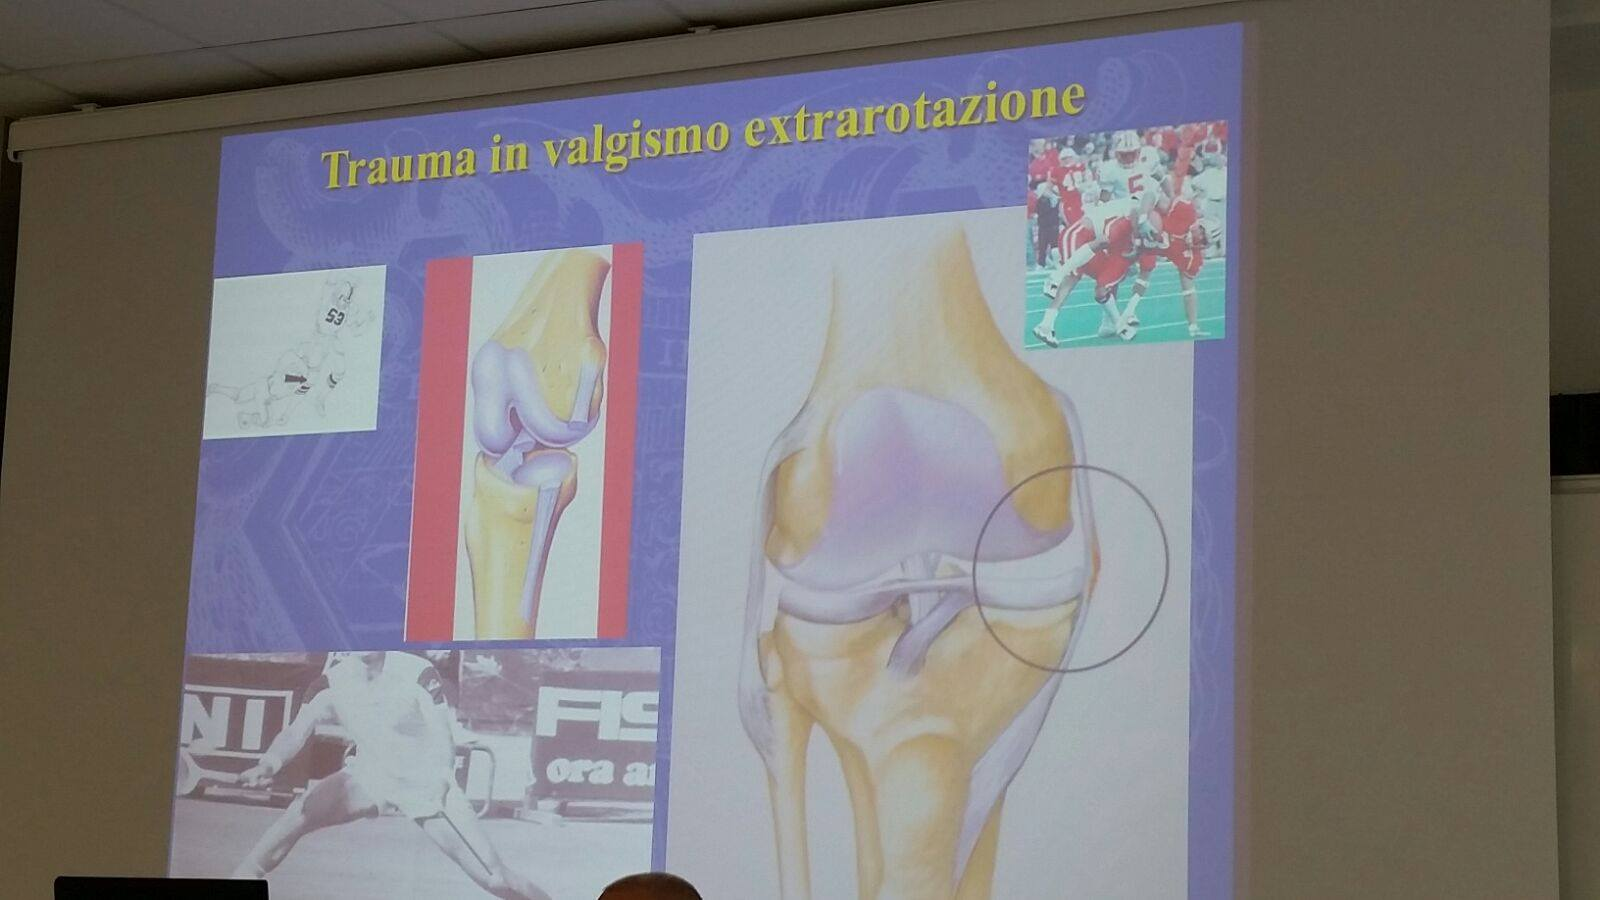
\includegraphics[width=0.4\textwidth]{008/image5.jpeg}
\end{figure}

La forma più frequente è il trauma in valgismo ed extrarotazione.(tipico trauma da inforcata degli sci). La lesione più lieve determina solo uno stiramento con ecchimosi della fascia e della capsula articolare.

In questi tipi di traumatismi la prima struttura che cede è il legamento collaterale mediale.

Se il trauma è ad alta energia può essere interessato anche il menisco interno, il legamento crociato anteriore e questa associazione è definita come triade tipica del trauma distorsivo del ginocchio.(chiamata triade interna) Nei traumi ad altissima energia ci può essere anche la lesione del crociato posteriore, del menisco esterno (pentade interna) e di tutti gli altri legamenti fino ad una lussazione del ginocchio con interessamento delle strutture vascolo nervose del
cavo popliteo.

\subsubsection{Trauma in varismo intrarotazione}

\begin{figure}[!ht]
\centering
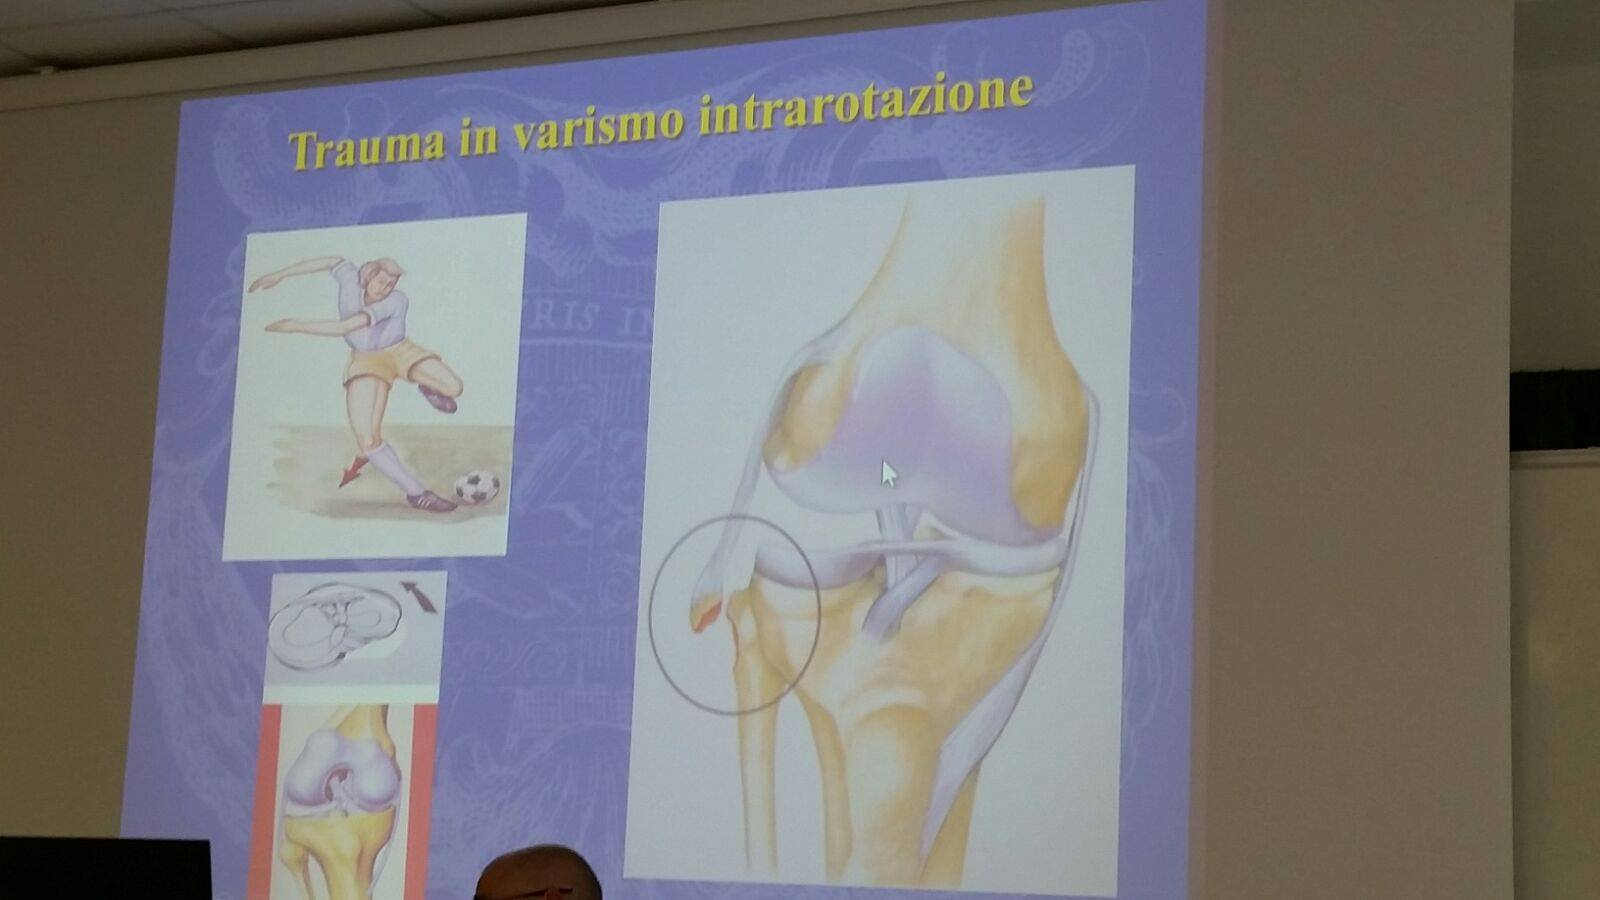
\includegraphics[width=0.4\textwidth]{008/image6.jpeg}
\end{figure}

Meno frequente è invece il trauma in varismo intrarotazione che è l'opposto di quello precedente. In questo caso la prima struttura che cede è il legamento collaterale laterale a cui può seguire la lesione del menisco esterno e una lesione del crociato anteriore. (triade esterna)

Anche qui se il meccanismo è dotato di altissima energia i crociati possono rompersi entrambi, può essere anche associata la lesione del menisco mediale, del collaterale mediale fino ad avere una lussazione del ginocchio. Possiamo avere in caso di trauma efficiente interessamento delle strutture del compartimento posteriore e delle strutture vascolari.

\subsubsection{Trauma in iperestensione}

\begin{figure}[!ht]
\centering
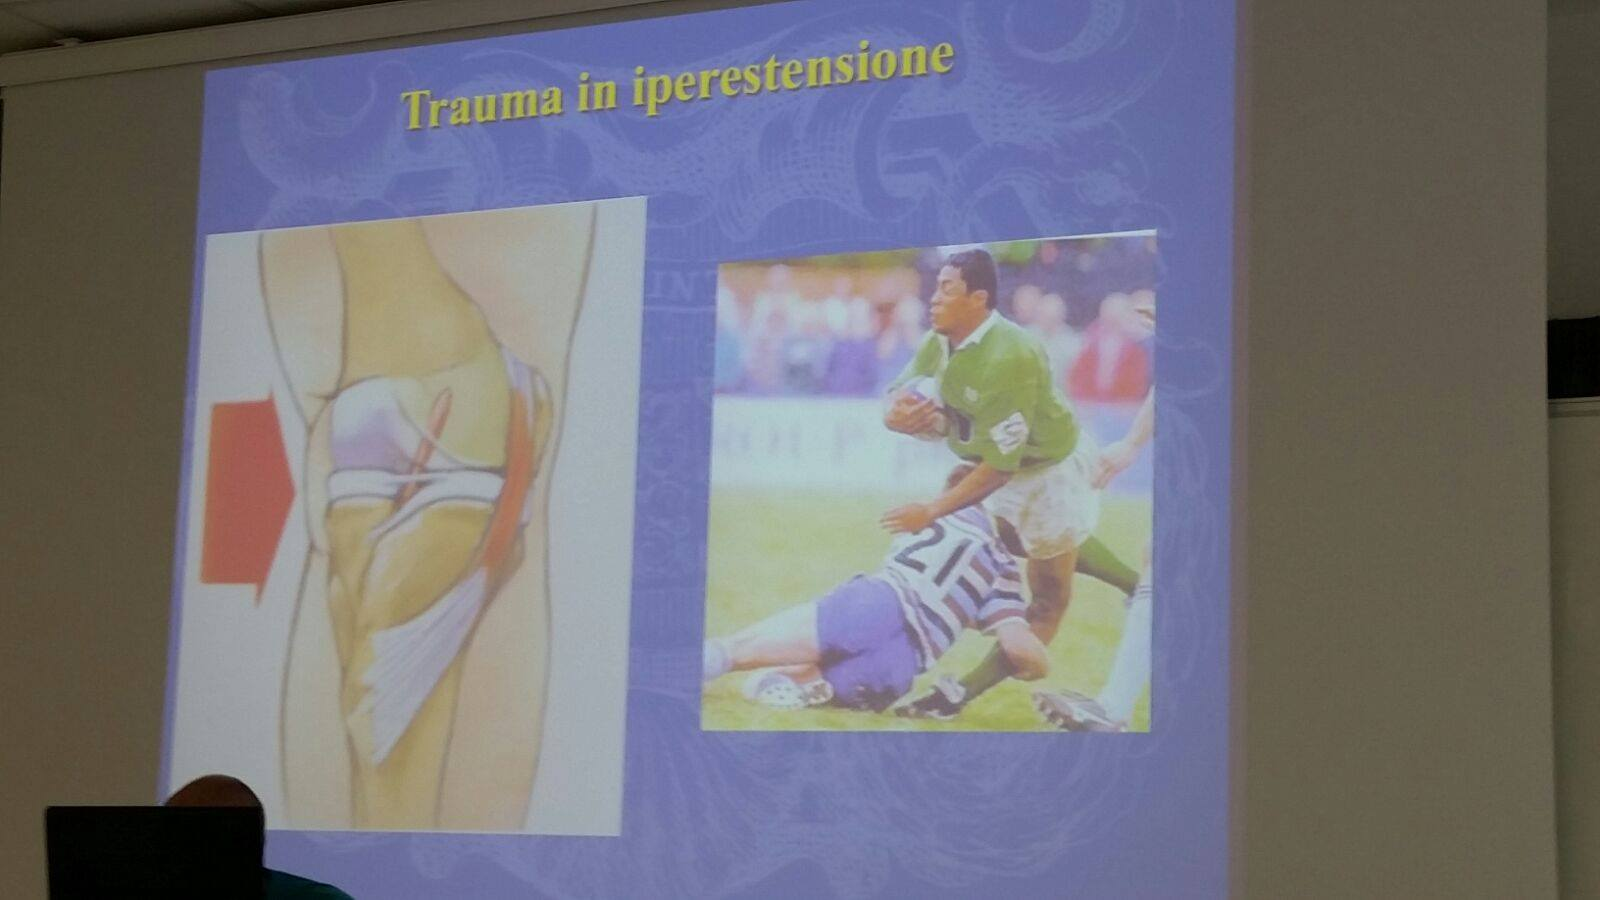
\includegraphics[width=0.4\textwidth]{008/image7.jpeg}
\end{figure}

Altro trauma presente soprattutto negli sport di contatto è il trauma in iperestensione. può capitare ai calciatori quando saltano di testa e atterrano male nella discesa, oppure per eventi traumatici diretti.

Trauma in cui la prima struttura ad essere interessata è il legamento crociato anteriore, a cui può seguire una lesione del crociato posteriore e poi lo stiramento di tutte le strutture comprese nel cavo popliteo (quindi lesioni vascolari e nervose associate).

\subsubsection{Trauma diretto sulla faccia anteriore della tibia}

\begin{figure}[!ht]
\centering
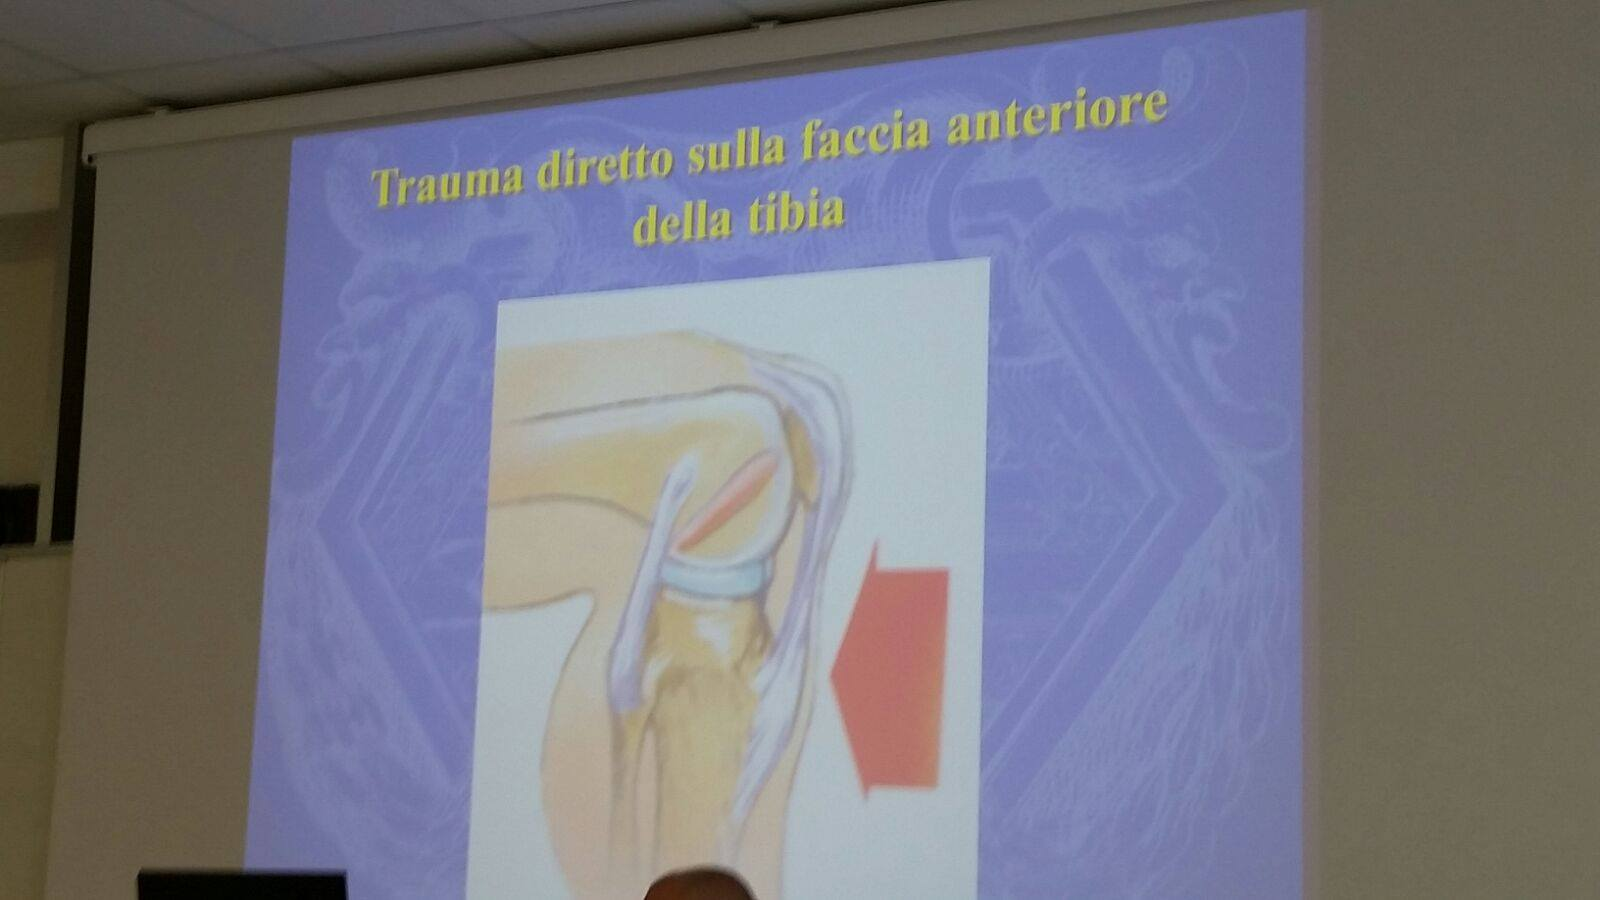
\includegraphics[width=0.4\textwidth]{008/image8.jpeg}
\end{figure}

Ultimo trauma è il trauma diretto sulla faccia anteriore della tibia. È la tipica ``lesione da cruscotto'': quando in macchina si fa un incidente si punta con i piedi e con il ginocchio si va a sbattere contro il cruscotto. In questo caso la tibia viene traslata in maniera acuta posteriormente e anche in questo caso le prime strutture che si lacerano sono i legamenti crociati (posteriore prima) a cui può seguire una lesione di tutte le strutture del cavo popliteo posteriore.

\subsection{Diagnosi e terapia}

Le lesioni croniche rappresentano l'esito di uno o più lesioni acute non riparate, per cui è essenziale riconoscere la qualità delle lesioni acute e trattarle nel modo più adeguato per garantire la loro cicatrizzazione ottimale, ed in generale si deve tenere a mente che cicatrizzano tutte le interruzioni non distanziate o approssimate con sutura, ad eccezione di quelle del crociato anteriore e della parte centrale dei menischi.

\subsubsection{Esame clinico}

\begin{itemize}
\item
  racconto anamnestico riguardo le modalità traumatiche, sensazione di "crack"
\item
  \textbf{atteggiamento antalgico in semiflessione} con impossibilità alla completa estensione,
\item
  \textbf{impotenza funzionale}
\item
  \textbf{tumefazione} ed eventuale presenza di \textbf{versamento
  intrarticolare} (se precoce, entro la prima ora è emartro; se tardivo, dopo 24-36 ore è idrartro)
\item
  \textbf{dolore} diffuso, più o meno accentuato e localizzato
\end{itemize}

Per quanto riguarda la sintomatologia, subito dopo al trauma, occorre soprattutto distinguere le distorsioni ``benigne'' da quelle gravi: le prime, infatti, guariscono con semplice riposo o immobilizzazione in gesso, mentre le seconde richiedono spesso un trattamento chirurgico.

Se dovesse capitarvi di fare i medici sportivi su un campo da gioco e un atleta si infortuna con una distorsione del ginocchio, dovrete capire sul campo, se questo atleta può tornare a fare attività sportiva subito o meno. Lo sportivo, se vuole riprendere subito a giocare probabilmente ha avuto un trauma distorsivo di lieve entità; se invece lamenta dolore al movimento, sensazione di instabilità (si può subito formare anche un versamento capsulare) e non chiede lui stesso di tornare, dobbiamo considerarlo un campanello d'allarme, perché gli sportivi di solito vogliono continuare a giocare (sopratutto se rugbisti!)
In quest'ultimo caso, si mette il ghiaccio ad intervalli, dopodichè si applica un bendaggio compressivo e si accompagna fuori dal campo

Gli indizi che indicano una lesione grave sono l'anamnesi di un trauma appoggiato, una sensazione immediata di ``crack'' e di lussazione del ginocchio, l'immediata impotenza funzionale ed il senso di instabilità permanente dopo il trauma. È quasi costante un versamento articolare ematico, che può mancare nelle lesioni più lievi, oppure in quelle più gravi dove l'ampia lacerazione della capsula lascia diffluire l'ematoma nei tessuti molli circostanti.

L'esame obiettivo è tipicamente ostacolato dal dolore, dalla contrattura muscolare antalgica, dall'ematoma e dall'edema che infiltrano i tessuti articolari e peri-articolari. Nelle lesioni più lievi, si può trovare un dolore palpatorio elettivo sul punto dove è lacerato un legamento collaterale, altrimenti il dolore è più diffuso.

\subsubsection{Esame obiettivo}
\begin{itemize}
\item[1.] La prima cosa da fare è valutare se c'è \textbf{tumefazione}, oppure no.
\item[2.] Secondo passaggio è il \textbf{test del ballottamento rotuleo}: si corica il paziente sul lettino, così che il liquido capsulare si raccolga al di sotto della rotula; dopodiché si preme la rotula verso il basso con due dita. Se è presente una raccolta di liquido, questo verrà spinto contro le pareti laterali, attorno alla rotula. Questa valutazione deve essere fatta anche nel ginocchio controlaterale; se non vi è versamento la rotula non avrà questo movimento.
\item[3.] Passaggio successivo, possibilmente in Pronto Soccorso (ambiente sterile), consiste nel fare un'\textbf{artrocentesi}, ossia uno svuotamento dell'articolazione del ginocchio, al fine di determinare anche le caratteristiche del liquido capsulare.
\end{itemize}
In un trauma distorsivo di un giovane atleta ci aspettiamo di trovare del sangue (\textbf{emartro}). A volte riscontriamo la presenza di gocce di grasso quando il trauma distorsivo è associato ad una frattura.

Se invece si trova un liquido sinoviale si parla di \textbf{idrartro}.
In alcuni casi si può trovare del pus all'interno del ginocchio, in questo caso si parla di \textbf{artrite
settica}.

L'iter diagnostico iniziale quindi è:
trauma distorsivo $\ge$ valutazioni in situ $\ge$ test del ballottamento $\ge$ artrocentesi $\ge$ riscontro di emartro (più frequente).

Dopo lo svuotamento del ginocchio il paziente starà subito meglio perché verrà meno la tensione legata alla tumefazione, successivamente si potranno eseguire test
specifici.

\subsubsection{Test specifici}

\begin{itemize}
\item
  reperi anatomici e ricerca dei punti dolorosi
\item
  \textbf{valutazione della stabilità articolare}:
\begin{itemize}
\item test per la stabilità \textbf{medio-laterale}: test in valgismo o abduzione, test in varismo o adduzione;
\item test per la stabilità \textbf{antero-posteriore}: test del cassetto anteriore, test del cassetto posteriore;
\end{itemize}
\item
  Jerk test;
\item
  \textbf{Lachman test;}
\item
  Test di gravità
\end{itemize}

L'esame si baserà prima di tutto sulla ricerca dei punti dolorosi:

\begin{itemize}
\item
  si valuterà inizialmente l'emirima articolare mediale, punto doloroso del \textbf{menisco mediale};
\item
  si palperà poi, l'emirima articolare laterale, punto doloroso del \textbf{menisco laterale};
\item
  infine si palperà il decorso del \textbf{legamento collaterale mediale} e \textbf{laterale}.
\end{itemize}

Di solito, il \textbf{LCM} fa male a livello del condilo femorale mediale, mentre il \textbf{LCL} fa male a livello della testa del femore.

\begin{itemize}
\item
  Si deve palpare anche l'integrità del \textbf{legamento rotuleo}: se si rileva una discontinuità palpatoria del legamento rotuleo il paziente non riuscirà ad estendere completamente il
ginocchio
\item
  A volte, associata alla lesione del legamento rotuleo, può esserci anche la rottura del \textbf{tendine} \textbf{quadricipitale}, ed anche in questo caso il paziente non sarà in grado di estendere il ginocchio.
\end{itemize}

\subsubsection{Test clinici per valutare stabilità del ginocchio}

Test per valutare stabilità laterale:

\begin{itemize}
\item
  Test in Valgismo (o in Abduzione), in cui si valuta l'integrità del legamento collaterale mediale; il test prevede di valgizzare il ginocchio esteso e flesso, e se è presente una lesione del legamento collaterale mediale, il ginocchio si aprirà di più rispetto al contro laterale.
\item
  Test in Varismo (o in Adduzione), che valuta l'integrità del legamento collaterale laterale, che anche in questo caso permette di valutare un angolo di apertura superiore al contro laterale.
\end{itemize}

Questi due test vengono fatti col ginocchio flesso di circa 20\textsuperscript{o}-30\textsuperscript{o} e
bisogna sempre confrontare i risultati col ginocchio contro laterale.
\\\\
Abbiamo quindi dei test che sono specifici per la valutazione della stabilità antero-posteriore:

\begin{itemize}
\item
  Test del Cassetto Anteriore e Posteriore, che serve a dimostrare una maggior lassità del ginocchio, appressabile manualmente e visibilmente durante l'esecuzione della manovra. Questi test vanno eseguiti flettendo il ginocchio a 90\textsuperscript{o}, si blocca la gamba del paziente e poi si trasla anteriormente (cassetto anteriore) e posteriormente (cassetto posteriore) l'epifisi prossimale tibiale, la quale ``scassetta'' in direzione in avanti (lesione del crociato anteriore) o in dietro (lesione del crociato posteriore).
  
\item
  Test di Lachman, è un altro test che si fa abitualmente per valutare l'integrità dei crociati, e si esegue senza bloccare il piede, con una mano si blocca l'estremità distale del femore e con l'altra di trasla anteriormente e posteriormente l'estremità prossimale della tibia. La sensazione che si riscontra se il paziente ha una lesione dei crociati è la mancanza di stop, cioè la mancanza di un blocco palpatorio con una maggior lassità dell'articolazione.
\end{itemize}

\subsubsection{Esami strumentali}

\begin{itemize}
\item
  radiografia in proiezioni ortogonali
\item
  ecografia
\item
  TC
\item
  RM
\item
  valutazione artroscopica
\end{itemize}

A questo punto abbiamo un quadro generale di questo paziente: il trauma che ha avuto, test meniscali positivi, se c'è stabilità o meno.
La prima cosa da fare, dopo una valutazione clinica accurata, è quella di richiedere una \textbf{radiografia} che può mettere in evidenza:

\begin{itemize}
\item
  se ci sono delle fratture associate al piatto tibiale,
\item
  se ci sono dei segni indiretti di lesione legamentosa, ad esempio l'avulsione dei legamenti nel punto in cui si inseriscono sull'osso (es. avulsione delle spine tibiali).
\end{itemize}
Dev'essere ripetuta spostando il ginocchio in più direzioni.

L'\textbf{ecografia} di solito non è indicata per i traumi distorsivi del ginocchio.

Può essere chiesta una \textbf{TC} qualora si sospetti una frattura non vista dalle lastre.

Ad ogni modo, l'esame principale per studiare le lesioni
capsulo-legamentose del ginocchio è la \textbf{risonanza magnetica} - che non è un esame di prima istanza in pronto soccorso - ma viene richiesto successivamente e normalmente viene eseguito in regime ambulatoriale Qualora voi facciate i medici di medicina generale, o comunque medici non specialisti in ortopedia, molto spesso vi capiterà di richiedere delle RM per mettere in evidenza delle fratture che non vengono evidenziate nelle radiografie, dal momento che la RMN è in grado di mettere in evidenza delle linee di frattura o dell'edema osseo post-traumatico che alle radiografie non sono visibili.

\subsubsection{Terapia}
\begin{itemize}
\item riposo, bendaggio elastico, crioterapia, FANS;
\item Immobilizzazione con apparecchi gessati, tutore;
\item Intervento chirurgico in artroscopia;
\item intervento chirurgico "a cielo aperto".
\end{itemize}
Uno dei referti più comuni, soprattutto nel giovane atleta, è la lesione del \textbf{legamento crociato anteriore}, e il trattamento consigliato è quello di ricostruire il legamento, ossia di sostituire il legamento lesionato con uno ex novo, di solito un legamento autologo prelevato dal proprio corpo.

Sono due i tipi di trapianti che possono essere effettuati:
\begin{itemize}
\item[1.] In passato veniva effettuato quasi sempre il \textbf{trapianto da tendine rotuleo}: si preleva una porzione di tendine rotuleo dal ginocchio omolaterale alla lesione che viene riposizionato al posto del crociato anteriore.
\item[2.] Oggi, è di uso comune l'utilizzo dei \textbf{tendini della zampa d'oca} (gracile e semitendinoso).
\end{itemize}

In tutti i casi, il trattamento consiste nella sostituzione e nella ricostruzione del legamento crociato anteriore, e la sostituzione avviene artroscopicamente.
\\\\
L'\textbf{artroscopia} è una tecnica chirurgica a minima invasività, che permette di guardare facilmente diversi tipi di lesioni articolari. Si posizionano tre cannule attraverso tre mini-incisioni a livello del ginocchio (Fig. 58). Con la prima incisione viene inserita una cannula che serve ad iniettare della soluzione fisiologica; le altre due incisioni si effettuano rispettivamente in posizione anteromediale ed antero-laterale: in una va inserita l'ottica, un apparecchio che serve a far vedere quello che c'è all'interno del ginocchio; nell'altra incisione invece, si inseriscono degli strumenti particolari, che serviranno ad effettuare la ricostruzione.

Per prelevare il tendine rotuleo, si asporta anche un frammento d'osso appartenente sia alla rotula che alla spina tibiale anteriore, lo si prepara con delle tecniche particolari, e poi viene impiantato al posto del legamento crociato anteriore e fissato con delle viti.
\\\\
Perciò:
\begin{itemize}
\item \textbf{Lesione del legamento crociato anteriore} (LCA): ricostruzione artroscopica, generalmente con tendine autologo. A volte, nelle lesione recidivanti - soprattutto negli atleti che magari hanno subito multipli e ripetuti infortuni ad entrambe le ginocchia - può essere indicato utilizzare:
\begin{itemize}
\item un legamento prelevato da cadavere (con tutte le limitazioni legate ad un trapianto eterologo),
\item dei legamenti sintetici.
\end{itemize}
Qualche giorno dopo l'intervento chirurgico il paziente può subito iniziare la fisioterapia ed il ritorno all'attività sportiva è variabile dai 4 ai 6 mesi. Le \textbf{lesioni meniscali} eventualmente associate, vengono trattate durante il medesimo atto chirurgico con delle \textbf{pulizie artroscopiche}:
\begin{itemize}
\item si fa una \textbf{meniscotomia parziale} quando le lesioni meniscali sono marginali;
\item in altri casi, soprattutto nelle plurinserzioni meniscali della capsula conviene effettuare una \textbf{sutura meniscale}.
\end{itemize}
Poiché il menisco ha una sezione triangolare, la parte più alta del triangolo è quella adesa alla capsula ed è anche quella più vascolarizzata, infatti si chiama
"\textbf{zona rossa} del menisco"; per cui, le lesioni vicino alla capsula possono guarire se suturate, mentre la parte più verso l'articolazione non è vascolarizzata ("\textbf{zona bianca} del menisco") per cui può essere ripulita.
\item Le \textbf{lesioni del collaterale mediale} (LCM) di solito non vengono trattate chirurgicamente, guariscono con un iniziale periodo di immobilizzazione associato a della fisioterapia e alla terapia fisica. Questo perché il LCM è un legamento nastriforme e, quando si rompe, i capi si riavvicinano, e ha un'ottima possibilità di cicatrizzazione spontanea.
\item Il \textbf{legamento collaterale laterale} (LCL), se ha lesioni importanti, deve essere riparato chirurgicamente dal momento che è un legamento cordoniforme, per cui in caso di rottura i due capi non si riavvicineranno mai.
\item Le \textbf{lesioni del crociato posteriore} (LCP) possono anche non essere operate, ad es. ci sono molti
calciatori che giocano con il crociato posteriore rotto. In questo caso, la lesione è vicariata da un ottimo tono-trofismo muscolare, anche se esistono delle tecniche chirurgiche artroscopiche o a cielo aperto che ne consentono la ricostruzione.
\end{itemize}

Nelle lesioni più lievi, limitate alla capsula, è sufficiente un'artrocentesi per estrarre il versamento ematico ed un'immobilizzazione gessata, e questa terapia è indicata anche nelle lesioni di media gravità (triadi) se il paziente è anziano. Nelle lesioni più gravi e nei pazienti giovani è invece indicata la riparazione chirurgica immediata, ed in generale i risultati sono buoni, ma dipendono dalla gravità delle lesioni, anche se in quelle gravi permane una certa lassità e non è possibile riprendere gli sports agonistici.

\subsection{Lesioni meniscali}

\begin{figure}[!ht]
\centering
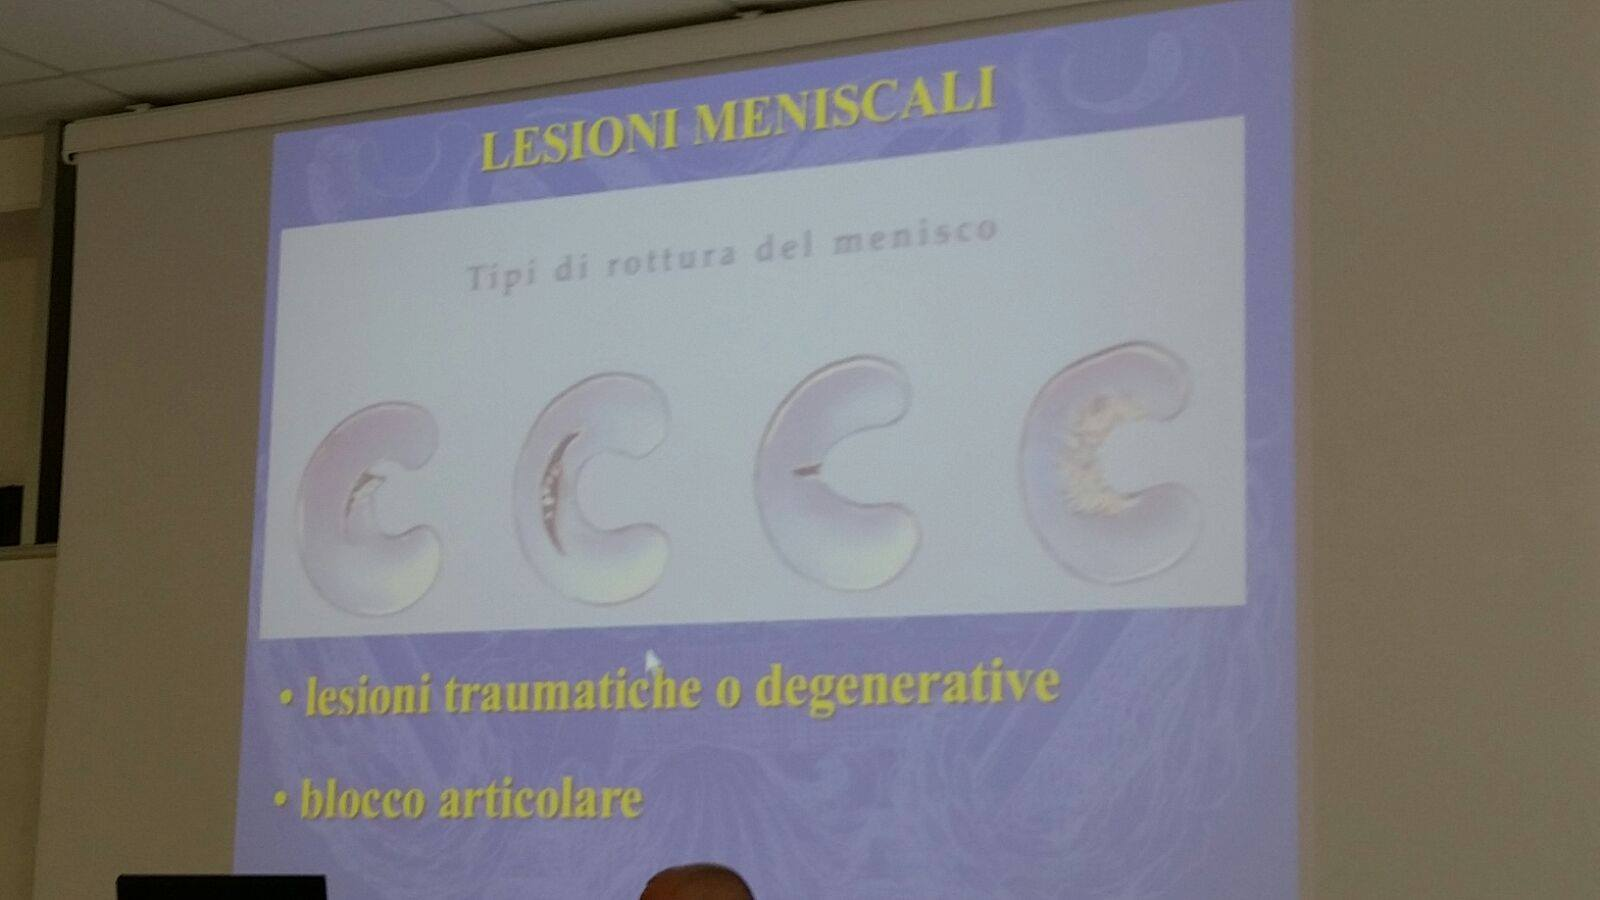
\includegraphics[width=0.4\textwidth]{008/image9.jpeg}
\end{figure}

Esistono poi le lesioni meniscali isolate o associate. Possono essere di 2 tipi:

\begin{itemize}
\item
  Le \textbf{lesioni traumatiche} sono di solito lesioni nette e vengono classificate in base al decorso della lesione: radiale, longitudinale, obliqua.
Le lesioni traumatiche dei menischi sono condizioni relativamente frequenti, e la lesione del menisco mediale è circa 7 volte più frequente di quella del menisco laterale, il quale viene lesionato o alterato in genere o come conseguenza di malformazioni congenite (menisco discoide) o per processi di degenerazione mixoido-cistica del menisco stesso. In generale, comunque, le lesioni meniscali sono più frequenti nel sesso maschile e nell'età adulta giovane, in particolare
negli sportivi, mentre sono rare nei bambini, fatta eccezione per le malformazioni congenite dei menischi.

Dal punto di vista patogenetico, la lesione traumatica di un menisco è sempre causata da un trauma distorsivo, mai da un trauma diretto.
Condizioni predisponenti alla lesione meniscale sono i fenomeni degenerativi del menisco, un pregresso trauma, che può aver determinato una lassità delle inserzioni meniscali o una piccola lacerazione del menisco. Durante il trauma distorsivo, il menisco viene rimane schiacciato tra il piatto tibiale ed il condilo femorale e non può seguire la tibia, per cui si fissura o si strappa dalle sue inserzioni tibiali o capsulari. Per quanto riguarda l'anatomia patologica, le lesioni traumatiche meniscali, in ordine di frequenza, sono le seguenti:

\begin{itemize}
\item
  Rottura Longitudinale, ``a manico di secchia'';
\item
  Strappo del Corno Posteriore;
\item
  Disinserzione del menisco dalla capsula;
\item
  Strappo del Corno Anteriore;
\item
  Rottura Trasversale.
\end{itemize}

\item
  Le \textbf{lesioni degenerative} invece non conseguono traumi distorsivi importanti, non danno rotture nette, ma danno una sorta di \emph{sfrangiamento} della superficie del menisco. Formano una sorta di ``pelucchi'' che sfioccano dalla superficie del menisco stesso. Dopo i 40 anni, a livello meniscale cominciano delle modificazioni artrosiche, con progressiva disidratazione della sua fibro-cartilagine che diventa meno elastica e compare una tipica fessurazione orizzontale, come una specie di ``slaminamento'' da usura.
\end{itemize}

Molto spesso nei traumi importanti il frammento del menisco si può ribaltare all'interno della gola femorale e questa lesione si chiama ``a manico di secchio". Può determinare un blocco articolare tra femore e tibia.

\subsection{Diagnosi e terapia}

Dal punto di vista clinico, la diagnosi di lesione meniscale si basa sull'anamnesi e su di un accurato esame clinico, mentre i radiogrammi non sono utili, e vengono in genere eseguiti solo per escludere lesioni
diverse da quella meniscale, mentre più utili sono l'artrografia, oggi poco usata, e l'artroscopia.

L'anamnesi rivela costantemente il trauma discorsivo, associato in genere ad altri elementi:

\begin{itemize}
\item
  Episodi di Blocco Articolare, infatti il paziente riferisce spesso che il ginocchio, una o più volte, si è ``bloccato'', quasi sempre in flessione, e tale blocco è causato da una lussazione di parte del menisco lacerato, verso il centro dell'articolazione, così che si va ad interporre tra le superfici articolari e ne impedisce la completa escursione. Il blocco spesso può essere risolto con opportune manipolazioni del ginocchio, che talvolta il paziente esegue da sé.
\item
  Senso di Cedimento del Ginocchio, che il soggetto avverte sotto carico e specialmente sotto sforzo.
\item
  Sensazione di Scroscio o di avere un corpo che si sposta all'interno dell'articolazione durante i movimenti del ginocchio.
\end{itemize}

L'esame obiettivo dimostra:

\begin{itemize}
\item
  dolore esattamente localizzato sull'emirima articolare mediale (se è interessato il menisco mediale) o laterale (se invece è interessato il menisco laterale), e questo segno è pressoché costante. Il dolore, nella stessa sede, si accentua forzando il ginocchio in estensione e ruotando la gamba, a ginocchio flesso verso l'esterno (per il menisco mediale) o verso l'interno (per le lesioni del menisco laterale); ed il dolore si accentua anche forzando il ginocchio, esteso, in varismo (per il menisco mediale) o in valgismo (per il menisco laterale), poiché queste manovre causano compressione del menisco leso.
\item
  Talora il ginocchio non può essere esteso completamente, vale a dire che è in fase di blocco, e questo segno, anche se appena accennato, ha valore diagnostico di certezza.
\item
  Talvolta si nota un lieve versamento intra-articolare ed inspessimento della membrana sinoviale, che reagisce allo stimolo meccanico rappresentato dalla fluttuazione del menisco rotto.
\item
  Se la lesione è già datata, è spesso presente ipotrofia del muscolo quadricipite femorale.
\end{itemize}

Utile è anche l'esecuzione di alcuni test meniscali puri, in cui il menisco provoca dolore nel momento in cui si iperestende o iperflettendo il ginocchio, e a seconda della localizzazione del dolore, mediale piuttosto che laterale, si può individuare l'eventuale lesione meniscale. Tra questi va ricordato

\begin{itemize}
\item
  il test di Apley, in cui si mette il paziente prono e si piega il ginocchio a 90\textsuperscript{o}, si prende la pianta del piede, si schiaccia contro al lettino e si fanno dei movimenti di intra/extra-rotazione del piede. Tutto questo determina una compressione del femore sulla tibia, cui consegue uno schiacciamento dei menischi che, se rotti, fanno male.
\end{itemize}

\subsubsection{Terapia ed Esiti delle Lesioni Meniscali}

La maggior parte delle lesioni meniscali si trattano in artroscopia, ed occorre sempre valutare globalmente le condizioni del ginocchio. Se, ad esempio, una rottura del menisco mediale si associa ad interruzione del crociato anteriore è controindicato asportare il menisco senza ricostruire il crociato, perché così si evidenzierebbe o aggraverebbe l'instabilità articolare. Nelle persone anziane, spesso di sesso femminile, se non vi è stato un vero e proprio trauma discorsivo, se il menisco non è chiaramente rotto, è molto probabile che il dolore sia dovuto ad un'iniziale artrosi femoro-tibiale mediale, e l'escissione del menisco, in tale condizione, non farebbe altro che peggiorare la condizione.

Regola fondamentale nella terapia è che la funzione del menisco deve essere rispettata: se la lesione consiste nel distacco del menisco della capsula o in una lacerazione della parte periferica del menisco, queste vengono suturate con filo riassorbibile, mentre le lacerazioni più centrali vengono trattate in artroscopia, rimuovendo la parte di menisco distaccata, lussata o fluttuante, e regolarizzando il bordo del menisco residuo, che viene conservato.

L'intervento in artroscopia ha il vantaggio di evitare o ridurre al minimo l'ospedalizzazione e di permettere una ripresa funzionale quasi immediata.

\subsection{Instabilità Croniche}

Quando la lesione non è ben guarita, inoltre, permane una certa instabilità cronica, che può manifestarsi con dolori che simulano una sindrome meniscale, e in questi casi sarebbe un grave errore asportare il menisco, poiché quest'operazione aggraverebbe la stabilità, che viene avvertita soprattutto nello scendere le scale, nel discendere per un terreno accidentato, nella corsa o sotto sforzo atletico. Le instabilità croniche possono essere generalmente suddivise in diversi tipi:

\begin{itemize}
\item
  Instabilità Anteriori, con cassetto anteriore, dovuto ad interruzione del crociato anteriore;
\item
  Instabilità in valgo-rotazione esterna;
\item
  Instabilità in varo-rotazione interna;
\item
  Instabilità Posteriori, da interruzione del crociato posteriore.
\end{itemize}

Per quanto riguarda la terapia e gli esiti del trattamento delle instabilità croniche, l'indicazione è difficile, ed il trattamento raramente è perfetto, e la lesione meniscale, spesso concomitante, va trattata a parte, ma tenendo sempre a mente che l'assenza di un menisco destabilizzerebbe ulteriormente il ginocchio. In generale, il crociato anteriore viene ricostruito con innesto prelevato dal tendine rotuleo o con un impianto sintetico, mentre la mancanza del crociato posteriore può essere in parte compensata retro ponendo sul piatto tibiale una parte del tendine rotuleo, mentre la lassità della capsula mediale o laterale può essere corretta con plastiche passive (della capsula stessa) o attive (dei tendini).
